\documentclass[11pt,a4paper]{report}
\usepackage[utf8]{inputenc}
\usepackage[french]{babel}
\usepackage[T1]{fontenc}
\usepackage{amsmath}
\usepackage{amsfonts}
\usepackage{amssymb}
\usepackage{makeidx}
\usepackage{svg}
\author{Frantzen Christian Marius Küpper}
\title{INFO-H-303 : Base de données\\
		Projet : Annuaire d'établissements horeca}
\begin{document}
\maketitle
\section*{Modèle entité-association}

\begin{figure}[h]
  \centering
  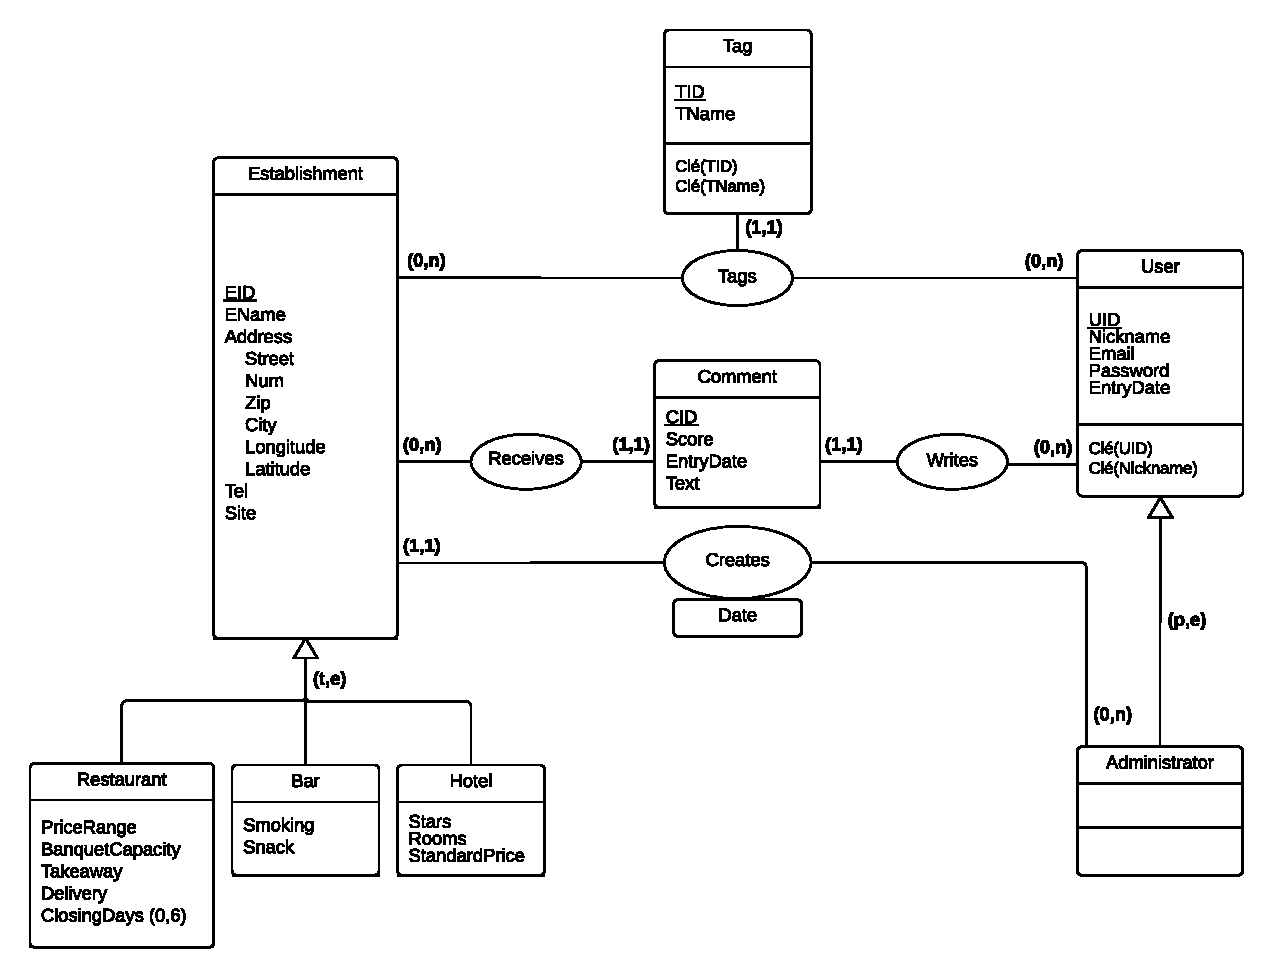
\includegraphics[width=\textwidth]{modelEA.pdf}
  \caption{Modèle entité-association}
\end{figure}


\subsection*{Contraintes d'intégrité}

\begin{itemize}
\item Un \textit{User} peut commenter plusieurs fois le même \textit{Establishment} à des dates différentes. 
\item Un \textit{User} ne peut pas apposer le même \textit{Tag} plusieurs fois sur le même \textit{Establishment}. 
\item L'\textit{EntryDate} d'un \textit{Comment} doit être strictement supérieure à l'\textit{EntryDate} du User qui le fait ainsi que l'\textit{EntryDate} de l'\textit{Establishment} sur lequel il est fait. 
\item Le \textit{Score} d'un \textit{Comment} est un entier compris entre 1 et 5.
\item Le nombre \textit{Rooms} d'un \textit{Hotel} doit être strictement positif. 
\item Le \textit{StandardPrice} d'un \textit{Hotel} doit être strictement positif. 
\item Le \textit{PriceRange} d'un \textit{Restaurant} doit être strictement positif. 
\item Le \textit{BanquetCapacity} d'un \textit{Restaurant} doit être positif. 
\end{itemize}
\subsection*{Remarques}
Si un \textit{Restaurant} ne veut pas organiser de banquet, il spécifie sa \textit{BanquetCapacity} comme étant 0.

\section*{Modèle relationnel}
\noindent
Establishment(\underline{EID},EName,Street,Num,Zip,City,Longitude,Latitude,Tel,Site,\underline{UID},EntryDate)
\begin{itemize}
\item UID référence User.UID\\
\end{itemize}
Restaurant(\underline{EID},PriceRange,BanquetCapacity,Takeaway,Delivery)
\begin{itemize}
\item EID référence Establishment.EID\\
\end{itemize} 
RestaurantClosingDays(\underline{EID},ClosingDay,Hour)
\begin{itemize}
\item EID référence Establishment.EID\\
\end{itemize}
Bar(\underline{EID},Smoking,Snack)
\begin{itemize}
\item EID référence Establishment.EID\\
\end{itemize}
Hotel(\underline{EID},Stars,Rooms,StandardPrice)
\begin{itemize}
\item EID référence Establishment.EID\\
\end{itemize}
User(\underline{UID},\underline{Nickname},Email,Password,EntryDate,Admin)\\ \\
%EstablishmentCreation.UNickname référence User.UNickname
%
%EstablishmentCreation.EName référence Establishment.EName
Comment(\underline{CID},\underline{UID},\underline{EID},Score,EntryDate,Text)
\begin{itemize}
\item UID référence User.UID
\item EID référence Establishment.EID
\item (UID,EID,EntryDate) est unique et donc également une clé de cette relation\\
\end{itemize}
Tag(\underline{TID},\underline{TName})\\ \\
EstablishmentTag(\underline{TID,EID,UID})
\begin{itemize}
\item TID référence Tag.TID
\item EID référence Establishment.EID
\item UID référence User.UID\\
\end{itemize}

\pagebreak
User.Admin est soit True soit False

Pour tout EstablishmentCreation il existe un Establishment

Pour le commentaire sur un établissement Comment.EntryDate <= EstablishmentCreation.EntryDate

Pour tout Establishment il existe soit un Restaurant, soit un Bar, soit un Hotel

0 <= Hotel.Stars <= 5

Hotel.Rooms >= 0

Hotel.StandartPrice > 0

Bar.Smoking est soit True soit False

Bar.Snack est soit True soit False

Restaurant.Delivery est soit True soit False

Restaurant.Takeaway est soit True soit False

Restaurant.BanquetCapacity >= 0

Restaurant.PriceRange >= 0

Comment.Score >= 0

Comment.EntryDate >= EstablishmentCreation 







\end{document}